\documentclass{article}

% \usepackage{ProbNum27}
% for camera ready:
\usepackage[final]{ProbNum27} 

% when publishing to a preprint service:
% \usepackage[preprint]{ProbNum27} 

% fallback if you cannot use hyperref (not recommended):
% \usepackage[nohyperref]{ProbNum27} 

% If you use natbib, leave the following three lines as they are:
\usepackage[round]{natbib}
\renewcommand{\bibname}{References}
\renewcommand{\bibsection}{\subsection*{\bibname}}
\bibliographystyle{abbrvnat}

% We recommend using cleveref:
\usepackage[capitalise,nameinlink]{cleveref}

\usepackage{kantlipsum}

\probnumtitle{Formatting Instructions for ProbNum \probnumyearpublic{}}
\probnumauthors{%
\name{Philipp Hennig}%
\affiliation{University of Tübingen, Tübingen AI Center, Germany}
\and%
\name{Alexandra Gessner}%
\affiliation{AstraZeneca, Barcelona, Spain}
\and%
\name{Motonobu Kanagawa}%
\affiliation{EURECOM, Sophia Antipolis, France}
\and%
\name{Jon Cockayne}%
\affiliation{University of Southampton, United Kingdom}%
\and%
\name{Toni Karvonen}%
\affiliation{LUT University, Finland}%
}


\probnumabstract{This document provides instructions for the preparation of submissions to the International Conference on Probabilistic Numerics \probnumyearpublic{}. The document itself conforms to the required styling and layout, and can be used as a template for submissions. The abstract should be limited to one paragraph, and should concisely summarize the research question, main results, and their relevance to the ProbNum community.}

\begin{document}

\section{General Layout}
\label{sec:general_layout}

Papers submitted to ProbNum \probnumyearpublic{} are limited to \textbf{at most 8 pages of main matter}, plus any additional pages needed for references and textual supplementary material. The conference chairs want to stress explicitly that papers are not required to run the full eight pages; shorter contributions are also invited. Note that reviewers are not required to consider supplementary material in their evaluation.

Papers must use the \LaTeX\ style provided with this template. It stipulates that paper should use \textbf{A4 page size}, with text laid out in two-column format using Computer Modern font. Each column is \the\columnwidth~wide, with a blank space of \the\columnsep~separating them. The text area is thus \the\textwidth~wide, which is hence also the width of double-wide figures.


\section{Text Macros}

\subsection{Equations and Mathematics}

\emph{All} equations must be numbered, e.g.\ by using the standard \texttt{equation} environment:
\begin{equation}
    \frac{\partial u(x,t)}{\partial t} + u(x,t) \cdot \frac{\partial u(x,t)}{\partial x} = \nu \cdot \frac{\partial^2 u(x,t)}{\partial x^2}.
\end{equation}

\subsection{Internal References}

For links within the text, we strongly recommend that you use the \texttt{cleverref} package. It allows, for example, to refer to \cref{sec:general_layout}.

\paragraph{Text Structure} All levels of headings available in the \LaTeX's \texttt{article} class (in other words, from section to paragraph) can be used within text if required. Note that excessive structure, especially in subsubsections, can be detrimental to the flow of your text.
All titles, headings and subheadings use title case.

\subsection{Citations}

Citations should use the author-year style, as defined in the style file. Use of \texttt{natbib} is recommended, but the package is not automatically loaded in the stylefile since it can cause compatibility problems with other packages (see the top of this example file for how to load it). When using natbib, note the difference between the \texttt{citep} and \texttt{citet} commands, which can used to cite names directly or passively. Make sure citations can be read as part of a sentence, as in the following example: First concepts of probabilistic computation were already suggested by \citet{laplace_prob}, but only recovered much later \citep[e.g.][]{ajne60:_nagra_tillaem,sard1963linear,larkin1972gaussian}.


\section{Figures and Tables}

\begin{figure}[b!]
    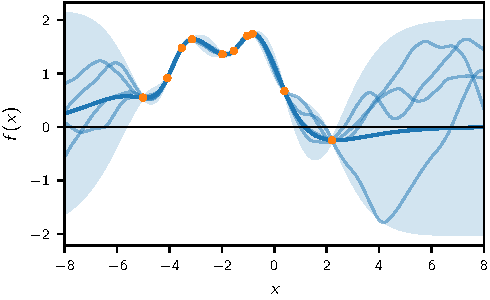
\includegraphics{fig/example_single_column.pdf}
    \caption{The \texttt{tueplots} package for \texttt{matplotlib} contains stylefiles for python plots. Its \texttt{probnum2025} bundle is recommended.}
    \label{fig:single-column}
\end{figure}

\subsection{Figures}

\begin{figure*}[t]
    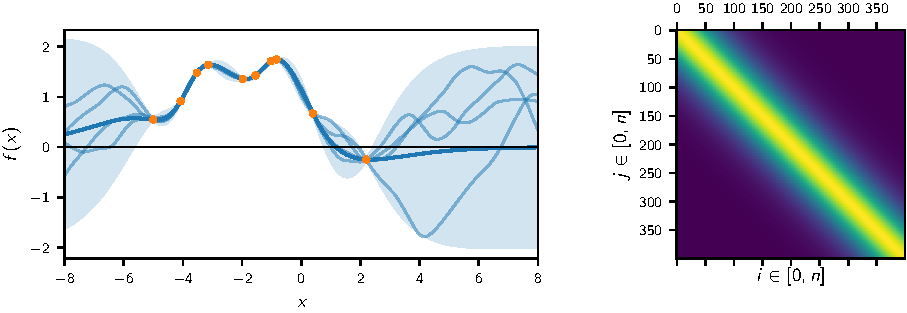
\includegraphics{fig/example_full_width.pdf}
    \caption{Both single-column (see \cref{fig:single-column}) and full-width figures like this one are possible. The \texttt{tueplots} package for \texttt{matplotlib} contains stylefiles for python plots. Its \texttt{probnum2025} bundle is recommended. Mathematical expressions in figure captions use sans-serif: $f(x)=x^2$.}
    \label{fig:full-width}
\end{figure*}

Figures should be included in the main text, placed at the top or bottom of the page if possible. There are two options for figures: single-column figures are \the\columnwidth~wide (\cref{fig:single-column} shows an example), while full-width figures are \the\textwidth wide (like \cref{fig:full-width}). For authors using python to generate plots, the \href{https://github.com/pnkraemer/tueplots/}{\texttt{tueplots}} package for \texttt{matplotlib} contains stylefiles. Use of its \texttt{probnum2025} bundle is recommended, and automates the process of creating figures in the correct style. To use the styles, first install the package with \texttt{pip install tueplots}, then add the following lines to your python script:
\begin{verbatim}
    import matplotlib.pyplot as plt
    from tueplots.bundles import probnum2025
    plt.rcParams.update(probnum2025())
\end{verbatim}
When creating figures, ensure not to explicitly set figure sizes, as this will override the style settings. For example, a simple figure can be created as follows:
\begin{verbatim}
    fig, ax = plt.subplots()
    x = np.linspace(0, 2*np.pi, 100)
    y = np.sin(x)
    ax.plot(x, y)
    fig.savefig('Figure_01.pdf')
\end{verbatim}
And such a figure can then be included in the \LaTeX\ document as shown in \cref{fig:single-column}. Note that the pdf is included in raw size, without the optional \texttt{width} argument. This ensures the figure's fonts match those of the document.

Authors who code in the julia language can use the\newline \href{https://github.com/nathanaelbosch/TuePlots.jl}{\texttt{tueplots.jl}} port, which contains an analogous
\begin{verbatim}
 \texttt{TuePlots.SETTINGS[:ProbNum25]}
\end{verbatim} pack. If you are using neither python nor julia, please adhere to the following guidelines:
\begin{itemize}
    \item Figures should be 240pts wide. The default \emph{height} is 148 (which is 240 divided by the golden ratio)
    \item Please use the open-source \textsf{Computer Modern Sans Serif} font for all strings, including axis labels, tickmarks, and axis titles (the same font is also used by this style for figure captions.)
    \item Axis labels and titles should be set to 9pt font size 
    \item Ticklabels and legend entries should use font size 7pt
    \item Colors can in principle be chosen freely. Authors should attempt to use accessible colormaps and palettes. Vaguely speaking, a blue/orange contrast can be perceived by a larger percentage of the population than a red/green one. It is \emph{not} necessary to use grayscale only, but important information can also be conveyed less ambiguous choices, like line widths and styles.
\end{itemize}

\subsection{Tables}


\begin{table}[b]\centering
\caption{Tables should be set in normalsize font if possible. If necessary, very wide tables can be set in scriptsize. They begin with a top rule, a header row, followed by a midrule. The entries of the table are concluded with a bottom rule. Maths in table captions uses sans-serif: $f(x) = x^2.$}
    \begin{tabular}{ll}
        \toprule
        Method           & Complexity         \\
        \midrule
        LU decomposition & $\mathcal{O}(N^3)$ \\
        Thomas algorithm & $\mathcal{O}(N)$   \\
        \bottomrule
    \end{tabular}
    \label{tab:1}
\end{table}

\subsection{Pseudocode}

Pseudocode, like actual programming languages, is difficult to standardize. However, as far as possible, authors are encouraged to use the layout provided by the \texttt{algpseudocodex} package loaded automatically with this stylefile, and which comes with some adaptations to style. \Cref{alg:1} provides an example.

\begin{algorithm}
    \begin{algorithmic}[1]
        \Procedure{Filter}{$m_{0},P_{0},A,Q,H,R,y$}
        \For{$t = 1,2,\dots,T$} \Comment{$\mathcal{O}(N)$}
        \State $m^- _{t} = A m_{t-1}$ \Comment{predictive mean}
        \State $P^- _{t} = A P_{t-1} A ^T + Q$ \Comment{pred.~cov.~$\mathcal{O}(|X|^3)$}
        \State $z = y - H m_t ^{-}$ \Comment{residual}
        \State $S = H P_t ^- H^T + R$ \Comment{innovation covariance}
        \State $K = P_t ^- H ^T S ^{-1}$ \Comment{gain. $\mathcal{O}(|y|^3)$}
        \State $m_t = m_t ^- + Kz$ \Comment{updated mean}
        \State $P_t = (I - KH) P_t ^-$ \Comment{updated covariance}
        \EndFor
        \State \Return{$(m_t,P_t),(m_t ^-, P_t ^-)$}
        \EndProcedure
    \end{algorithmic}
    \caption{An example algorithm (the Kalman filter). Note the line numbers and sans-serif maths in captions: $f(x) = x^2$.}
    \label{alg:1}
\end{algorithm}

The rest of this text is filler material to create three pages of document.

\kant[1-5]

\section*{Acknowledgements}

Acknowledgements of funding or other support should be placed in an unnumbered section at the end of the main text. Leave this section empty during anonymous review.

\bibliography{references}


\appendix


\section{Place your appendices here}

Place additional material in the appendix, such as additional experiments or proofs.
There is no page limit for the appendices, but as stated in the main paper, reviewers are not required to consider them in their evaluation.
Use the same formatting instructions for the appendices as for the main paper.


\section{Another appendix}
Again, the rest of this text is filler material.

\kant[1-2]



\end{document}